\documentclass[conference, a4paper]{IEEEtran}
\IEEEoverridecommandlockouts
\usepackage{cite}
\usepackage{amsmath,amssymb,amsfonts}
\usepackage{graphicx}
\usepackage[font=footnotesize]{caption}
\usepackage{textcomp}
\usepackage{xcolor}
\usepackage{url}
\usepackage{booktabs}
\setlength{\parskip}{6pt}
\setlength{\floatsep}{0pt}
\setlength{\textfloatsep}{6pt}
\setlength{\intextsep}{6pt}
\usepackage{geometry}
\geometry{a4paper, top=2cm, bottom=2.5cm, left=1.6cm, right=1.6cm}
\newtheorem{proposition}{Proposition}
\begin{document}

\title{On the Exploitability of Fair Multi-Agent\\ Reinforcement Learning}

\makeatletter
\def\@IEEEauthorblockNfont{\fontsize{11pt}{13pt}\selectfont}
\def\@IEEEauthorblockAfont{\fontsize{10pt}{12pt}\selectfont}
\makeatother

\author{\IEEEauthorblockN{Can Savc\i}
\IEEEauthorblockA{\textit{Independent Researcher}\\
\.{I}zmir, Turkey \\
savcisavcican@gmail.com}}

\maketitle

\begin{abstract}
Fair cooperative multi-agent reinforcement learning (MARL) methods such as SOTO
and FEN train agents to optimize a fairness-inducing welfare function (e.g.\ the
Generalized Gini Welfare) over the team's returns, so that no agent is left
behind. These methods implicitly assume that \emph{every} agent cooperates in
being fair. We show that this assumption is a vulnerability: a single
self-interested agent can \emph{exploit} a welfare-optimizing team, because fair
agents sacrifice their own utility to raise the worst-off and a best-response
defector appropriates that surplus. In rivalrous allocation games the effect is
\emph{exact by construction}: when the welfare-optimal policy is to yield, a lone
claimant takes everything, so the free-ride factor equals the team size $N$ (these
serve as analytical sanity checks, and a faithful SOTO learner reproduces the same
$N\times$ outcome, confirming it learns the yield policy). Our empirical evidence
comes from settings with genuine learned contention: a collision-prone claim game
($3.0\times$) and a FEN-style Matthew-effect gridworld ($1.9\times$, with seed
variance), where the Jain index falls sharply. We further show that a natural
\emph{policy-level} defense (reciprocity with adversarial co-training)
\emph{fails}---provably, in the all-or-nothing model---because cooperators cannot
deny a free-rider without wasteful levelling-down. Finally we show that an
egalitarian (worst-off-first) allocation rule, \textbf{EKREM}, restores
incentive-compatibility (free-ride $\approx 1$ for $N\ge 4$) by taking allocation
\emph{out of the agents' hands}; we are explicit that this sidesteps, rather than
solves, the harder problem of \emph{decentralized} robustness.
\end{abstract}

\renewcommand{\IEEEkeywordsname}{Keywords}
\begin{IEEEkeywords}
multi-agent reinforcement learning, fairness, exploitability, incentive
compatibility, social welfare
\end{IEEEkeywords}

\section{Introduction}
Cooperative multi-agent reinforcement learning (MARL) increasingly targets not
only efficiency but \emph{fairness}: in traffic control, resource allocation, and
networking, optimizing aggregate return alone can starve individual agents.
Leading fair-MARL methods---FEN~\cite{jiang2019fen} and
SOTO~\cite{zimmer2021soto}---reframe the objective as a fairness-inducing welfare
function over the agents' returns, typically the Generalized Gini Welfare (GGF),
which weights worse-off agents more heavily and thus rewards equity as well as
efficiency.

These methods are designed and evaluated under an implicit assumption: that all
$N$ agents are jointly optimizing the shared welfare. In many deployments this is
optimistic. Consider fair traffic-signal control where one intersection's
controller is upgraded to greedily minimize its own delay, or fair bandwidth
sharing where one client maximizes its own throughput: the remaining controllers
still ``play fair,'' yielding capacity to the worst-off. Agents may be controlled
by different stakeholders, or one agent may simply be trained (or retrained) to
maximize its own return. We ask a basic robustness question that the fair-MARL
literature has largely left implicit: \emph{what happens to a welfare-optimizing
fair team when a single member is self-interested?}

We find the answer is sharp. Because fair (team-oriented) agents
\emph{sacrifice} their own utility---yielding resources to raise the worst-off---a
self-interested agent can free-ride on that sacrifice. We make this concrete with
a best-response analysis and report three contributions:
\begin{itemize}
\item \textbf{A diagnostic.} A single best-response defector exploits a
GGF-welfare team, collapsing the Jain index toward $1/N$. In the yield-based
allocation games the over-share is $\rho{=}N$ \emph{by arithmetic} (analytical
sanity checks; a faithful SOTO learner reproduces the same $N\times$, confirming
it learns the welfare-optimal yield policy). The substantive evidence is in
settings with \emph{learned} contention---a collision-prone claim game
($3.0\times$) and a Matthew-effect gridworld ($1.9\times$, real seed variance).
\item \textbf{A negative result.} The obvious policy-level defense---reciprocity
with adversarial co-training---fails. We prove (for the all-or-nothing model) that
cooperators cannot deny a free-rider efficiently; denial requires wasteful
levelling-down, which an efficiency--equity objective rightly refuses.
\item \textbf{A positive result (with a caveat).} \textbf{EKREM} instantiates the
classic egalitarian (worst-off-first) allocation rule inside the MARL loop:
resources go by \emph{need}, so greedy claims earn nothing and
incentive-compatibility is restored (free-ride $\approx 1$ for $N\ge 4$). We are
explicit that it works by \emph{removing agents' control over allocation}---it
sidesteps, not solves, decentralized robustness.
\end{itemize}

\section{Background and Related Work}
\textbf{Welfare-based fair MARL.} Given per-agent (discounted) returns
$\mathbf{J}=(J_1,\dots,J_N)$, fair-MARL maximizes a Schur-concave welfare
$W(\mathbf{J})$ that is increasing (efficiency) and favors equity. A common choice
is the Generalized Gini Welfare $W(\mathbf{J})=\sum_{k} w_k J^{\uparrow}_k$, where
$J^{\uparrow}$ sorts returns ascending and $w_k$ is decreasing, so the worst-off
receive the largest weight~\cite{siddique2020ggf}. FEN~\cite{jiang2019fen} uses a
hierarchical controller over sub-policies driven by a fair-efficient reward;
SOTO~\cite{zimmer2021soto} learns a \emph{Self-Oriented} sub-network (own return)
and a \emph{Team-Oriented} sub-network (welfare), annealing behavior from
self-oriented to team-oriented over training.

\textbf{Fairness under self-interest.} A complementary line incentivizes fairness
among self-interested agents via \emph{mediators}: Ivanov et al.~\cite{ivanov2023mediated}
restore cooperation through an incentive-compatible (IC) mediator that respects
agents' boundaries, and Dodwadmath and Maghsudi~\cite{dodwadmath2025mediators}
elicit fair leaders via mediators (their JAM-QL framework). These methods
\emph{deter} free-riding through IC rather than learned reciprocity, and so are
closely related to our positive result. Our \emph{question}, however, is dual and,
to our knowledge, not previously isolated: taking an existing \emph{cooperative}
fair learner as given, how fragile is it when one member defects? We
\emph{stress-test} welfare-optimizing fair methods with a best-response defector
and quantify their exploitability.

\textbf{Social dilemmas and free-riding.} The vulnerability we expose is a
fairness-specific instance of free-riding in sequential social
dilemmas~\cite{leibo2017ssd} and common-pool problems: a contributor's sacrifice
can be appropriated by a non-contributor. Whereas social-dilemma MARL studies the
\emph{emergence} of cooperation, we study how an explicitly fairness-seeking
objective \emph{creates} an appropriable surplus---the utility team-oriented agents
forgo to raise the worst-off---and who captures it.

\textbf{Mechanism design and fair division.} Our fix is not a new allocation rule
but the import of a classic one. Allocating to the worst-off is the egalitarian /
leximin principle of fair division~\cite{moulin2003fair}, and making truthful
(here, need-revealing) behavior optimal is the goal of mechanism
design~\cite{nisan2001amd}. EKREM instantiates this known incentive-compatible
egalitarian mechanism \emph{inside} the MARL loop.

\textbf{Exploitability and best response.} In competitive MARL, a policy's
\emph{exploitability} is the gain of a best response to it. We import this lens to
\emph{cooperative} fairness: we hold the fair team fixed and train a best-response
defector, treating its realized over-share as an exploitability measure for the
fairness mechanism.

\section{Problem Formulation}
We consider $N$ agents acting over an episode of $T$ steps. Let $u_i \ge 0$ be
agent $i$'s accumulated utility (resources collected) and
$\mathbf{u}=(u_1,\dots,u_N)$. A \emph{fair} team maximizes a Schur-concave welfare
$W(\mathbf{u})$ that is increasing in each $u_i$ (efficiency) and favors equity. We
use the Generalized Gini Welfare
\begin{equation}
W(\mathbf{u}) = \sum_{k=1}^{N} w_k\, u^{\uparrow}_k, \qquad
w_1 > w_2 > \dots > w_N > 0,
\end{equation}
where $u^{\uparrow}$ sorts $\mathbf{u}$ ascending, so the worst-off agent carries
the largest weight. We report fairness with Jain's
index~\cite{jain1984fairness},
$\mathrm{Jain}(\mathbf{u})=\big(\sum_i u_i\big)^2 / \big(N\sum_i u_i^2\big)\in(0,1]$
($1$ = perfectly fair), and the Gini coefficient.

\textbf{Threat model.} A fair team of $N$ policies is trained to maximize
$W(\mathbf{u})$. We then \emph{freeze} the team, replace one agent by a
\emph{defector}, and train the defector to maximize its \emph{own} utility
$u_{\mathrm{def}}$ as a best response to the frozen teammates. We quantify the
exploit by the \emph{free-ride factor}
\begin{equation}
\rho = \frac{u_{\mathrm{def}}}{\bar{u}}, \qquad
\bar{u} = \tfrac{1}{N}\textstyle\sum_i u_i,
\end{equation}
the defector's utility over the equal (fair) share. $\rho = 1$ is exactly fair;
$\rho = N$ means the defector took everything. A fairness method is
\emph{exploitable} if a best-response defector attains $\rho \gg 1$, and
\emph{robust} (incentive-compatible) if $\rho \approx 1$.

\section{Environments}
\textbf{Allocation games and a Matthew-effect gridworld.}
\emph{(i) claim}: each step one resource is available; agents choose
\textsc{Claim}/\textsc{Yield}; a sole claimer wins it, collisions waste it.
\emph{(ii) donate}: as claim, but if all yield the resource auto-routes to the
worst-off (so fair play is to yield and let the needy collect).
\emph{(iii) matthew}: among claimers the \emph{richest} wins, capturing FEN's
rich-get-richer dynamic.
\emph{(iv) FEN gridworld}: a 2D grid with one (respawning) resource; an agent's
movement speed scales with its wealth (rich move every step, poor
intermittently), so fair play requires the rich to yield.

In every game, action $1$ is the \emph{self-interested} act (claim/keep) and $0$
is to \emph{defer} (yield/donate). Under GGF the optimal joint policy is the same
across games---``act selfishly only when you are the worst-off''---which a fair
team must learn, and which a defector violates.

\section{Experimental Setup}

\begin{figure*}[t]
\centering
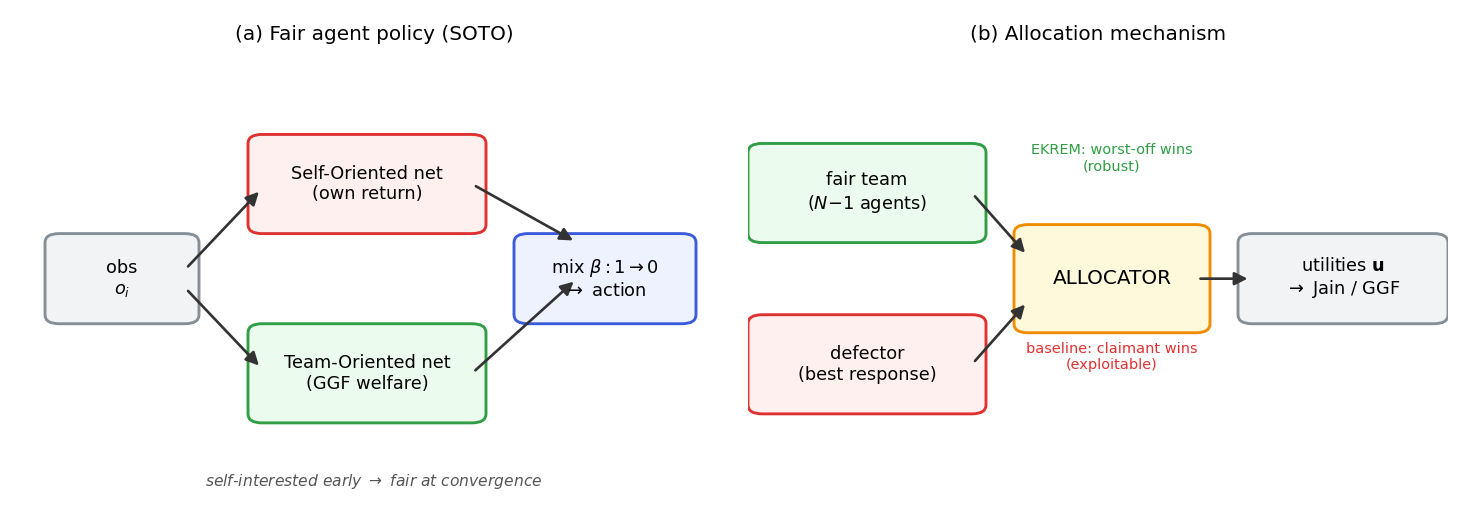
\includegraphics[width=0.96\linewidth]{fair_arch.png}
\caption{Overview. (a) The fair agent policy: a SOTO learner combines a
Self-Oriented sub-network (own return) and a Team-Oriented sub-network (GGF
welfare), annealing from self-interested to fair over training. (b) The
allocation mechanism turns agents' requests into utilities: the \emph{baseline}
awards the resource to the claimant (exploitable by a defector), whereas
\textbf{EKREM} awards it to the worst-off (need-based, robust).}
\label{fig:arch}
\end{figure*}

\noindent Fig.~\ref{fig:arch} gives an overview of the policy architecture and the
allocation mechanism. \textbf{Fair team.} We train two fair learners. (i)~A simplified shared-policy
GGF learner: a single policy controls all agents and is optimized to maximize
$W(\mathbf{u})$. (ii)~A faithful \textbf{SOTO}: a Self-Oriented sub-network
(own-return objective) and a Team-Oriented sub-network (GGF objective), with the
behavior probability annealing from self-oriented to team-oriented over training;
at convergence ($\beta{=}0$) the team is purely team-oriented, i.e.\ fair.

\textbf{Defector.} After the fair team converges we freeze it, designate one agent
as the defector, and train its policy to maximize its own utility against the
frozen teammates---a best response.

\textbf{Optimization.} All policies are two-layer MLPs trained with
REINFORCE~\cite{williams1992reinforce} (Adam, $512$ parallel episodes). Each agent
observes its own and the team's utility statistics (its rank/being-worst-off) and,
in the gridworld, its position relative to the resource. The gridworld uses a
dense GGF-increment reward ($r_t = W(\mathbf{u}_t)-W(\mathbf{u}_{t-1})$) so that
navigation is learnable; the abstract games use the terminal welfare. Unless
noted, $N{=}4$ and results are averaged over $3$ seeds.

\section{Welfare-Optimizing Fairness is Exploitable}
Table~\ref{tab:exploit} reports the exploit at $N{=}4$ (Fig.~\ref{fig:bars}
visualizes it against EKREM). We separate two kinds of result.

\textbf{Analytical sanity checks (donate, matthew, SOTO).} In the yield-based
games the welfare-optimal joint policy is for everyone to yield (the resource
auto-routes to the worst-off). A defector that always claims is then the
\emph{sole} claimant and takes the resource every step, so $\rho{=}N$ \emph{by
arithmetic}---not by learning. This is exactly why these entries are
zero-variance. The faithful \emph{SOTO} run is the same fact reproduced by a real
learner: its $4.0\times$ confirms that SOTO converges to the GGF-optimal yield
policy, \emph{not} that the exploit is independently nontrivial. We therefore treat
these as sanity checks rather than empirical evidence.

\textbf{Empirical evidence (claim, gridworld).} The substantive results come from
settings with genuine learned contention. In \emph{claim} (no auto-routing,
collisions waste the resource) the defector reaches $3.0\times$ rather than
$4.0\times$: on steps where the worst-off cooperator also claims, the collision
wastes the resource and the defector \emph{forfeits} it, so the number is shaped by
the contention dynamics, not just $N$. The \emph{FEN gridworld} ($1.9\times$, with
real seed variance) is the strongest test: agents must navigate, the defector
cannot be everywhere, and fairness still falls from $0.88$ to $0.67$.

\begin{table}[t]
\caption{Exploitability at $N{=}4$. A single best-response defector vs.\ a trained
fair team. Free-ride $=$ defector utility / fair share.}
\label{tab:exploit}
\centering
\begin{tabular}{lccc}
\toprule
Environment & Fair-team Jain & Free-ride & Jain w/ defector \\
\midrule
donate            & 1.00  & $4.0\times$ & 0.25 \\
claim             & 0.998 & $3.0\times$ & 0.43 \\
matthew           & 1.00  & $4.0\times$ & 0.25 \\
FEN gridworld     & 0.88  & $1.9\times$ & 0.67 \\
\midrule
faithful SOTO (donate) & 1.00 & $4.0\times$ & 0.25 \\
\bottomrule
\end{tabular}
\end{table}

\begin{figure}[t]
\centering
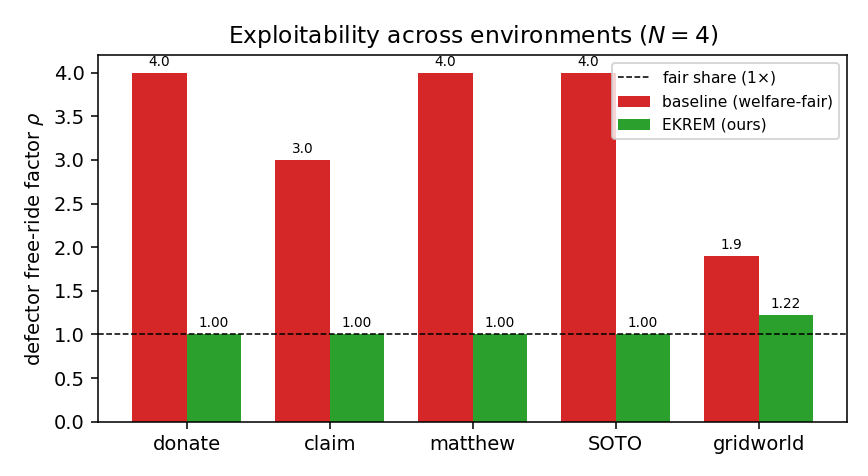
\includegraphics[width=0.95\linewidth]{fair_exploit_bars.png}
\caption{Defector free-ride factor $\rho$ per environment ($N{=}4$). A single
self-interested agent free-rides $1.9$--$4\times$ against the welfare-fair
baseline; EKREM brings every case back toward the fair share ($\rho\approx 1$).}
\label{fig:bars}
\end{figure}

\textbf{The exploit scales with team size.} Fig.~\ref{fig:scaling} shows that in
the donate game the free-ride factor grows essentially as $N$ (the defector takes
everything, so its share is $N\times$ fair) and the post-defector Jain falls as
$1/N$: at $N{=}16$ a single self-interested agent drives fairness to $0.06$. The
larger and more cooperative the team, the more there is to exploit.

\begin{figure}[t]
\centering
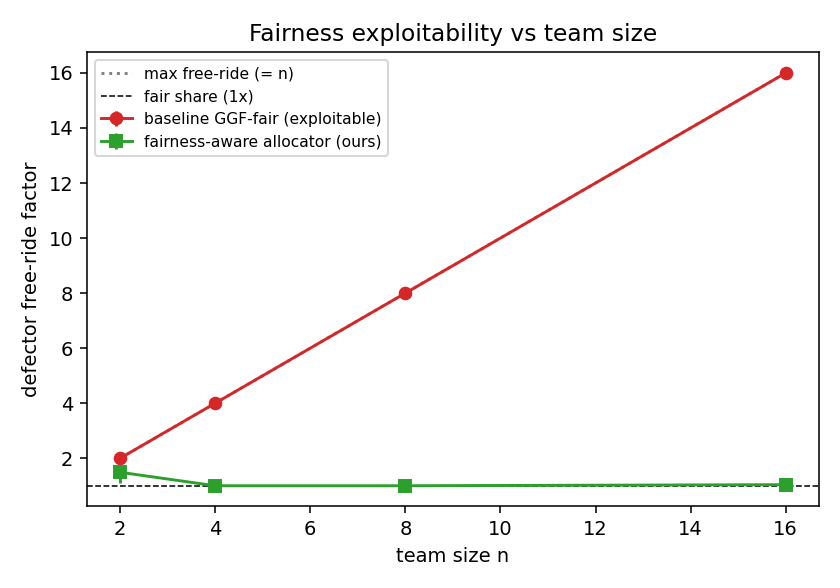
\includegraphics[width=0.92\linewidth]{fair_solidify.png}
\caption{Free-ride factor vs.\ team size $N$. The baseline welfare-fair team is
exploited along the diagonal (free-ride $\approx N$); EKREM (our need-based
allocator) stays flat at $\approx 1$. Mean over 3 seeds.}
\label{fig:scaling}
\end{figure}

\begin{table}[t]
\caption{Scaling with team size $N$ (donate game, 3 seeds). The baseline exploit
grows as $\approx N$ and fairness collapses as $\approx 1/N$; EKREM holds
$\rho\approx 1$ and Jain $\approx 1$ for $N\ge 4$, with a residual at $N{=}2$
($\rho{=}1.49$; see text).}
\label{tab:scaling}
\centering
\begin{tabular}{ccccc}
\toprule
 & \multicolumn{2}{c}{Baseline} & \multicolumn{2}{c}{EKREM} \\
\cmidrule(lr){2-3}\cmidrule(lr){4-5}
$N$ & free-ride $\rho$ & Jain & free-ride $\rho$ & Jain \\
\midrule
2  & 2.00  & 0.50  & 1.49 & 0.77 \\
4  & 4.00  & 0.25  & 1.00 & 1.00 \\
8  & 8.00  & 0.125 & 1.00 & 1.00 \\
16 & 16.00 & 0.063 & 1.04 & 0.998 \\
\bottomrule
\end{tabular}
\end{table}

\section{Why a Policy-Level Defense Fails}
A natural fix is to make cooperation \emph{conditional}: agents detect an
over-claimer (a reciprocity feature) and are adversarially co-trained against a
best-response defector so they learn to contest it. This \emph{fails}: a freshly
trained defector still free-rides $\approx 4\times$ and the contesting degrades
the team's own fairness.

The reason is structural, and we can state it precisely.

\begin{proposition}[Futility of policy-level defense]
Consider a rivalrous resource allocated each step to a claimant (sole claimant
wins; a collision wastes the resource), against a defector that claims at every
step. Then for \emph{any} cooperator policies, at each step either (i) some
cooperator claims, colliding with the defector so the resource is wasted, or
(ii) no cooperator claims and the defector wins. In both cases the cooperators
obtain zero of that resource. Hence the only way to reduce the defector's utility
is to force collisions, which wastes the resource without benefiting cooperators;
a GGF-maximizing team is therefore indifferent between yielding and contesting.
\end{proposition}

\noindent Intuitively, cooperators cannot \emph{capture} the surplus they would
deny the defector---denial is pure levelling-down, which an efficiency--equity
objective correctly refuses. Policy-level reciprocity thus has no efficient
leverage; robustness must come from the allocation \emph{mechanism}, which can
redirect the contested resource to a needy cooperator rather than wasting it. We
emphasize that the proposition is specific to \emph{all-or-nothing waste}; under
partial allocation or graded contention the ``collision $\Rightarrow$ total waste''
premise breaks and the conclusion need not hold (Sec.~IX).

\section{EKREM: A Need-Based Fair Allocator}
\textbf{EKREM} instantiates the classic egalitarian (worst-off-first / leximin)
allocation rule~\cite{moulin2003fair} inside the MARL loop. Rather than ``whoever
grabs the resource gets it,'' the resource is allocated by \emph{need}: to the
worst-off agent (overall, or among claimers). The rule itself is not new---it is
the standard incentive-compatible egalitarian mechanism~\cite{nisan2001amd}---and
that is precisely the point. A defector's greedy claims are honored only when it is
genuinely worst-off (exactly when receiving is fair), so over-claiming earns
nothing, while efficiency is preserved because the resource still goes to a
cooperator. Fig.~\ref{alg:ekrem} states the rule. We stress that EKREM achieves
this by \emph{removing agents' control over allocation}: once a central need-based
allocator decides, policies no longer determine who receives the resource, so there
is nothing left to exploit (see Sec.~IX).

\begin{figure}[t]
\centering
\fbox{\begin{minipage}{0.92\linewidth}
\footnotesize
\textbf{EKREM allocation step}\\[2pt]
\textbf{Input:} utilities $\mathbf{u}$; requesters $C$; fair share $s=t/N$\\[1pt]
1.\ $E \leftarrow \{ i \in C : u_i < s \}$ \ (requesting \emph{and} below fair share)\\
2.\ \textbf{if} $E \neq \emptyset$ \textbf{then} $w \leftarrow \arg\min_{i \in E} u_i$ \ (neediest eligible)\\
3.\ \textbf{else} $w \leftarrow \arg\min_{i} u_i$ \ (worst-off overall; no waste)\\
4.\ $u_w \leftarrow u_w + 1$
\end{minipage}}
\caption{The EKREM allocation step: resources flow by \emph{need}, so a claim
succeeds only when the claimer is genuinely worst-off.}
\label{alg:ekrem}
\end{figure}

Table~\ref{tab:fix} shows EKREM holds the free-ride factor at $\approx 1$ and Jain
at $\approx 1$ across the abstract environments and against faithful SOTO, and
substantially mitigates the gridworld exploit ($1.90{\to}1.22$, fair-team Jain
preserved at $0.85$, three seeds; per-seed in Table~\ref{tab:perseed}). Because allocation tracks
\emph{need} rather than \emph{grabbing}, a defector's claims are honored only when
it is genuinely worst-off---exactly when receiving is fair---so over-claiming earns
nothing and incentive-compatibility is tight for $N\ge 4$ ($\rho{\approx}1$,
Table~\ref{tab:scaling}). The exception is $N{=}2$ ($\rho{=}1.49$, Jain $0.77$):
with only two agents a defector can deliberately drive itself below the fair share,
become the genuine worst-off, claim and overshoot before the partner recovers, so
the need-gate oscillates rather than binding tightly. We report $N{=}2$ as a
residual (as with the gridworld); the mechanism is tight for $N\ge 4$.

\begin{table}[t]
\caption{EKREM restores incentive-compatibility.
Free-ride factor with a best-response defector (lower is better; $1$ = fair).}
\label{tab:fix}
\centering
\begin{tabular}{lcc}
\toprule
Environment & Baseline & EKREM \\
\midrule
donate / matthew (abstract) & $4.0\times$ & $1.0\times$ \\
faithful SOTO               & $4.0\times$ & $1.0\times$ \\
FEN gridworld (3 seeds)     & $1.90\times$ & $1.22\times$ \\
\bottomrule
\end{tabular}
\end{table}

\section{Discussion and Limitations}
\textbf{Centralization.} EKREM allocates by need and therefore requires (an
estimate of) agents' utilities---the same global-information assumption already
made by SOTO's welfare gradient. It effectively moves fairness from the
\emph{policy} to the \emph{mechanism}: rather than hoping self-interested agents
behave fairly, the allocation rule makes greedy behavior unrewarding. Where a
trusted allocator (a scheduler, a base station, a market clearing house) exists,
this is a practical and provably incentive-compatible fix.

\textbf{The hard open problem.} Proposition~1 applies to the all-or-nothing
rivalrous model: a contested resource is either won by a single agent or wasted.
Under that model a decentralized cooperator cannot deny a free-rider except by
wasteful levelling-down, which an efficiency--equity objective refuses. We
\emph{conjecture}, but do not prove, that the difficulty extends more broadly;
with partial allocation or graded contention resolution the premise breaks and
decentralized cooperators may regain leverage (e.g., by partially contesting).
Making welfare-fair teams non-exploitable with only local information and action
is, to our knowledge, open; we offer the centralized EKREM as an upper bound that
decentralized methods should aim to match.

\textbf{Scope.} Our environments are deliberately controlled---small
resource-allocation games and a compact gridworld---to isolate the mechanism;
larger gridworlds, continuous control, and multiple simultaneous defectors are
natural extensions, as is a coalition of colluding defectors. We expect the
qualitative story to persist: any objective that has cooperators sacrifice for the
worst-off creates an appropriable surplus.

\textbf{Takeaway for fair-MARL evaluation.} Fair-MARL methods are typically
evaluated on the fairness they \emph{achieve under full cooperation}. We argue they
should additionally be reported on the fairness they \emph{retain under
self-interest}---an exploitability audit---since the former can be high while the
latter is near-zero.

\section{Conclusion}
Welfare-optimizing fair MARL is exploitable: a single self-interested agent can
free-ride on the team's sacrifice by up to $N\times$, and the effect worsens with
scale and holds against a faithful SOTO implementation. Policy-level reciprocity
cannot fix this, for a structural reason; EKREM, a simple need-based allocation
mechanism, can. We hope the exploitability lens encourages fair-MARL methods to be evaluated
not only for the fairness they achieve under full cooperation, but for the
fairness they \emph{retain} under self-interest.

\section*{Code Availability}
All code (environments, SOTO, EKREM, and experiments) and the \LaTeX{} source are
available at \url{https://github.com/highcansavci/ekrem-fair-marl}.

\appendices
\section{Implementation Details}
All policies are two-layer $\tanh$ MLPs (width $32$ for the abstract games, $64$
for the gridworld) trained with REINFORCE and Adam (learning rate
$3\times10^{-3}$) using $B{=}512$ parallel episodes. Episodes last $T{=}100$--$200$
(abstract games) or $T{=}80$ (gridworld). The GGF weights are
$w_k \propto (N{-}k{+}1)$ over ascending-sorted utilities, placing the largest
weight on the worst-off. The fair team trains for $400$--$800$ updates and the
best-response defector for the same. The faithful SOTO uses separate Self- and
Team-Oriented MLPs and anneals the self/team mixing probability $\beta$ from $1$
to $0$ over the first $70\%$ of training; we evaluate at $\beta{=}0$ (purely
team-oriented). All reported numbers average $3$ seeds.

\section{Per-seed Results}
The abstract games and the faithful SOTO are effectively deterministic at
convergence (zero seed variance), which is why Tables~\ref{tab:exploit}
and~\ref{tab:fix} report exact $4.0\times$/$1.0\times$ values. The gridworld, with
stochastic movement and respawns, varies mildly; Table~\ref{tab:perseed} gives
the per-seed free-ride factor, confirming the exploit ($\approx1.9\times$) and
EKREM's mitigation ($\approx1.2\times$) are reproducible.

\begin{table}[h]
\caption{FEN gridworld free-ride factor $\rho$ per seed ($N{=}4$).}
\label{tab:perseed}
\centering
\begin{tabular}{lcccc}
\toprule
Allocator & seed 0 & seed 1 & seed 2 & mean \\
\midrule
Matthew (baseline) & 1.91 & 1.91 & 1.87 & 1.90 \\
EKREM (need-based) & 1.17 & 1.25 & 1.24 & 1.22 \\
\bottomrule
\end{tabular}
\end{table}

\bibliographystyle{IEEEtran}
\bibliography{refs}

\end{document}
